\section{Behavior Model V2} \label{sec:bmv2}


Before we start to introduce our experiment system setup. We want to introduce the behavior model we use. Bmv2~\cite{bmv2} is a software switch recommended by p4.org and ONF. It is still in develop stage but already support many protocols such as P4 runtime, grpc protocol to accept commands and can be deployed different P4 program through SDN controller in runtime.

Bmv2 is an opensource software written in C++, and obey to P4 specification.
There are two versions of P4, P4-14 and P4-16, published in 2014 and 2016
 respectively. However, bmv2 does not only support P4-16. Version 2 means that they redesign this pervious behavior model. In behavior model, we have to recompile the whole program if we deploy a new P4 program. Fortunately, bmv2 fixed this problem and add some other fancy features. Now the P4 compiler will compile P4 program into JSON format and deploy into bmv2 without recompile it.

\begin{figure}[tbh]
    \centering
    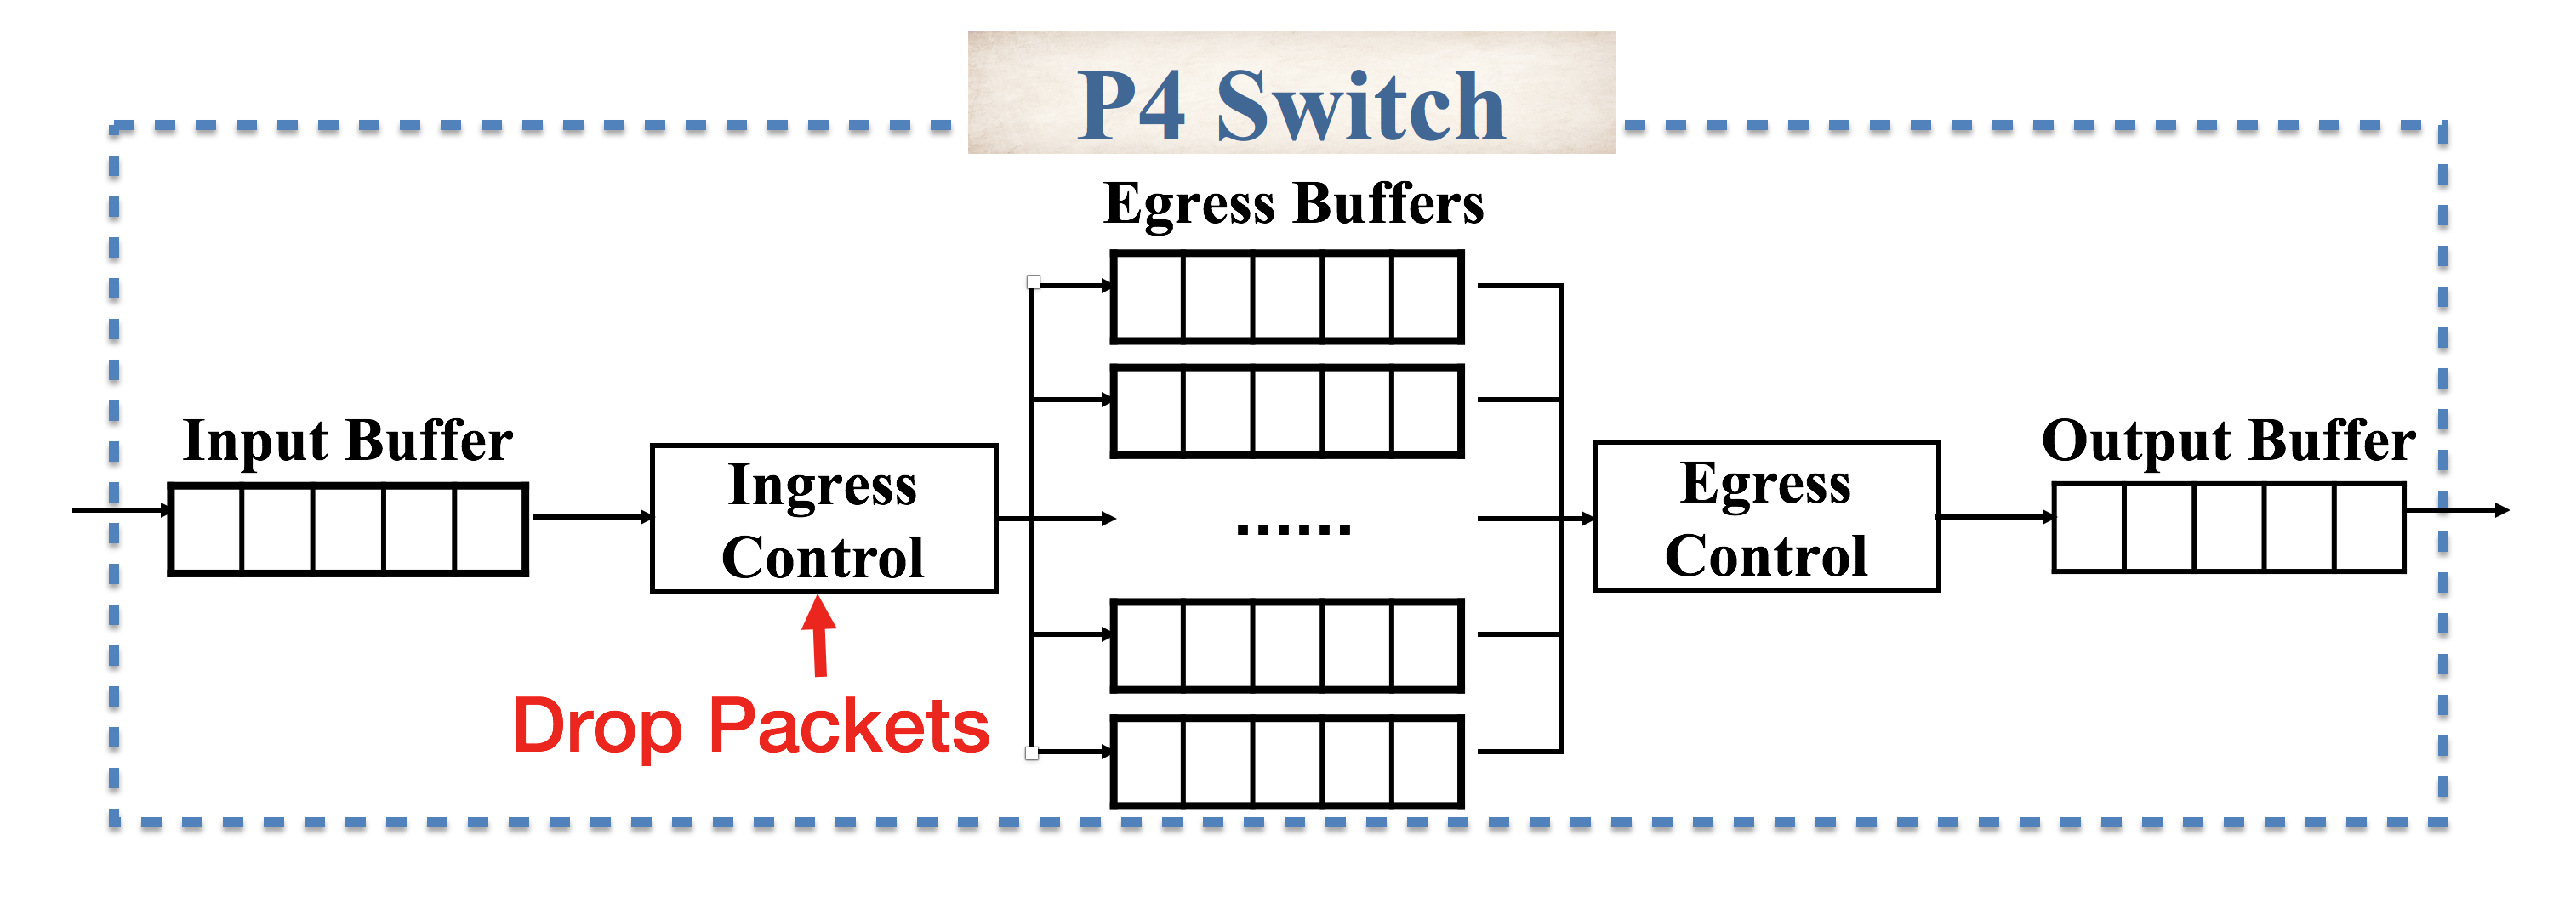
\includegraphics[width=.50\textwidth]{fig/bmv2Buffer.png}
    \caption{Buffers in bmv2}
    \label{bmv2Buffer}
\end{figure}

Fig. ~\ref{bmv2Buffer} shows all the buffer inside a bmv2. Please note that there are many interfaces connected to the buffer. Every packet comes into this MANE will first push into the input buffer. After our P4 program finish parsing the packet. Our ingress control will determine which port should this packet be forwarded and push into the right buffer relate to the port. In the ingress control, we detect the size of queue related to the forwarding egress buffer, and implement the three logics we mentioned before. If this packet pass the ingress control, it will be push into egress buffer and add some information such as source MAC address and reduce Time-to-Live value. Finally it will push to the interface attached to that port and leave MANE.

